\chapter{Cenário avaliado}
\label{CAP4}

Neste capítulo, é apresentado o ambiente Apache Hadoop que foi idealizado, no qual é baseado em uma metodologia exploratória e experimental. Esse ambiente busca prover um auxílio ao usuário para que ele possa realizar testes antes de montar um ambiente real.

O ambiente Apache Hadoop consiste em alguns \textit{softwares} gratuitos nos quais foram necessários realizar os \textit{downloads}, tais como: Ubuntu-server 16.04, java-8, Hadoop-2.9.1, Ubuntu-Desktop-16.04, virtual-box e o kali-Linux-x64. A figura \ref{Fig:EstruturaGeraldoAmbiente}, ilustrada no primeiro capítulo tenta dar uma visão geral do ambiente proposto. Os \textit{downloads} dos \textit{softwares} citados anteriormente são ferramentas essenciais para o desenvolvimento deste trabalho, o procedimento de instalação também é bastante simples, porém, um pouco demorado considerando o \textit{hardware} da máquina principal e tendo em vista que tudo estará dependendo apenas de uma máquina.

\begin{comment}
De inicio foi instalado o virtual-box na máquina local, em seguida foi criado uma máquina virtual com o ubuntu-server na sua instalação padrão com a instalação do openSSH Server que servirá para comunicação entre os nós do cluster. Após isso, foi instalado o java na versão 8, em seguida basta clonar essa máquina criada e escolher ela como o master e os demais como os slaves. Após isso foi necessário criar uma chave pública e um usuário e senha para cada nó.
\end{comment}

\section{Processo de instalação}

O processo de criação de uma máquina virtual com o \textit{software} virtual-box é bem simples, basta abrir o \textit{software} e depois clicar no botão 'novo', após isso é só escolher o nome e a quantidade de memória que deseja alocar para a máquina virtual. Com isso, basta seguir os procedimentos de instalação do sistema operacional, tais como, idioma, hora, usuário e senha.

\subsubsection{Instalação do Ubuntu Server}

Um cluster pode ser criado com qualquer sistema operacional, inclusive ele pode conter máquinas com diferentes sistemas operacionais, visto que, a comunicação é realizada pela rede via ssh, sendo assim, optou-se pelo sistema operacional Ubuntu server, pois o mesmo é gratuito e de código aberto. 

Ao concluir a instalação do Ubuntu server, é necessário fazer algumas outras instalações no sistema operacional, tais como, o java e o openSSH. Concluindo essas instalações é necessário desabilitar o ipv6 para poder utilizar o endereço 10.0.0.0 como \textit{network}. Para desabilitar o ipv6 bastar ir no caminho /etc/sysctl.config e adicionar as seguintes linhas:

\begin{figure}[htbp!] \begin{center}
	% fbox faz uma borda ao redor do seu argumento
    \fbox{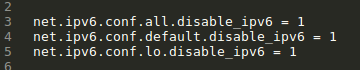
\includegraphics[width=0.80\linewidth]{figures/disableIpv6}}
    \caption{Desabilitando o Ipv6}
	\small{Fonte - (próprio autor, 2018)}
	\label{Fig:Desabilitando o Ipv6}
	\end{center} \end{figure}

%http://blog.aloi.com.br/?p=284


Tendo o java instalado, o openSSH instalado e o ipv6 desabilitado, precisa-se criar uma chave para o SSH, que permite a conexão sem precisar digitar senha. Para criar a chave foi utilizado o comando: 'ssh-keygen -t rsa -P "" '. Após gerar a chave pública basta copiar para um arquivo chamado \textit{authorizedKeys}, isso tudo significa que está máquina aceitará a conexão de outra máquina que tenha a chave privada. Então, até este momento a configuração entre as máquinas do cluster está configurada. A próxima etapa é a instalação e configuração do \textit{framework} Apache Hadoop. 

\subsubsection{Instalação do framework Apache Hadoop}

Assim que concluir a instalação do Ubuntu server e as configurações necessárias, basta realizar o \textit{download} do Apache Hadoop, que pode ser encontrado no repositório da unicamp no seguinte link: \url{http://ftp.unicamp.br/pub/apache/hadoop/core/stable/}.

Logo que o \textit{download} for conluído é necessário editar o arquivo de configuração do usuário, chamado de .bashrc, neste arquivo são adicionados as variáveis de ambiente do Hadoop ao PATH, com as seguintes linhas de código: \\

\begin{figure}[htbp!] \begin{center}
	% fbox faz uma borda ao redor do seu argumento
    \fbox{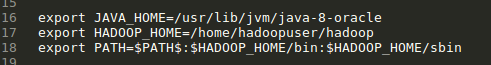
\includegraphics[width=0.80\linewidth]{figures/variaveisBashrc}}
    \caption{Adicionando variáveis do Apache Hadoop ao path}
	\small{Fonte - (próprio autor, 2018)}
	\label{Fig:Adicionando variaveis do hadoop ao path}
	\end{center} 
\end{figure}


Concluindo essa etapa, basta clonar a máquina \textit{master} criada e renomear as demais máquinas, transformando-as em \textit{slaves}, pois isso economiza tempo e as configurações já estão todas certas. No momento de realizar o clone, deve-se selecionar o \textit{checkbox} para reinicializar o endereço MAC da nova máquina, após isso basta configurar o IP de cada \textit{slave} para que eles fiquem na mesma faixa de IP, ou seja, na mesma rede.

Após isso, começa a instalação do Apache Hadoop, as configurações própriamente dita, entrando no seguinte caminho, hadoop/etc/hadoop e editando o arquivo hadoop-env.sh, pois ele é comum tanto para o \textit{master} quanto para os \textit{slaves}, neste arquivo é necessário colocar o caminho que o java esta instalado na máquina, para descobrir isso, basta digitar o comando "env | grep JAVA", neste caso a saída foi "JAVA\_HOME=/usr/lib/jvm/java-8-oracle".

O \textit{framework} Apache Hadoop contém diversos arquivos de configuração, esses arquivos são do tipo XML e especificam como o \textit{framework} irá conduzir suas tarefas. Para configurar o Apache Hadoop foi necessário editar alguns arquivos XML, tais como: 

\begin{itemize}

\item \textbf{Core-site.xml:} Este arquivo define as configurações de qual host será o \textit{master} no cluster Hadoop.

\begin{comment}
\begin{center}
	\lstinputlisting[caption = {core-site}, label=teste]{figures/core-site.xml}
\end{center}
\end{comment}

\begin{comment}
\begin{figure}[htbp!] 
	\begin{center}
	% fbox faz uma borda ao redor do seu argumento
	\fbox{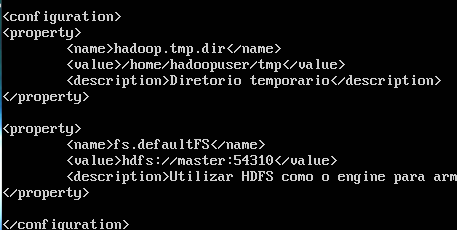
\includegraphics[width=0.80\linewidth]{figures/configCore-site}}
	\caption{Configuração do Core-site.xml}
    \small{Fonte - (proprio autor, 2018)}
	\label{Fig:Configuração do core-site.xml}
	\end{center} 
\end{figure}
\end{comment}

\item \textbf{Hdfs-site.xml:} É o \textit{filesystem} e nele são configurados as quantidades de replicações que o Hadoop HDFS deve fazer, onde estão localizados os metadados que o namenode utiliza para gerenciar o cluster e onde estão sendo armazenados os arquivos dentro do HDFS.

\begin{comment}
\begin{figure}[htbp!] 
	\begin{center}
	% fbox faz uma borda ao redor do seu argumento
	\fbox{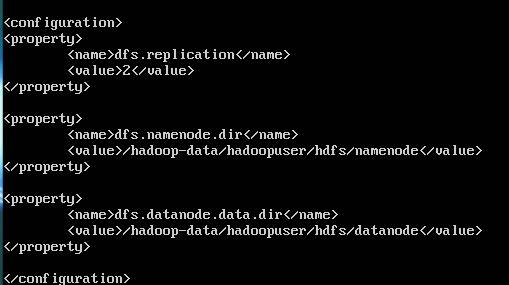
\includegraphics[width=0.80\linewidth]{figures/confighdfs-site}}
	\caption{Configuração do Hdfs-site.xml}
	\small{Fonte - (proprio autor, 2018)}
	\label{Fig:Configuração do hdfs-site.xml}
	\end{center} 
\end{figure}
\end{comment}

\item \textbf{Mapred-site.xml:} Este arquivo não existe por padrão, copia-se ele do mapred-site.xml.template e depois edita. Este arquivo define as configurações responsável por qual \textit{framework} que vai rodar os \textit{Jobs} do MapReduce, neste caso é o Yarn. Como o Yarn funciona com o conceito de container, é necessário alocar memória tanto para a operação de \textit{map} quanto para operação de \textit{reduce}.

\begin{comment}
\begin{figure}[htbp!] 
	\begin{center}
	% fbox faz uma borda ao redor do seu argumento
	\fbox{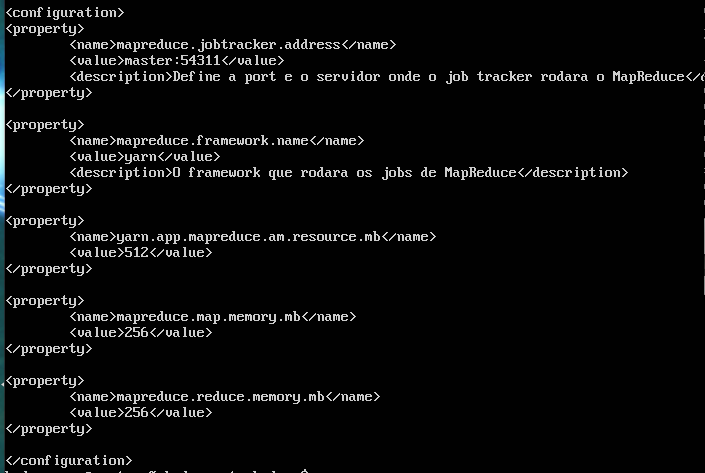
\includegraphics[width=0.90\linewidth]{figures/configmapred-site}}
	\caption{Configuração do mapred-site.xml}
	\small{Fonte - (proprio autor, 2018)}
	\label{Fig:Configuração do mapred-site.xml}
	\end{center} 
\end{figure}
\end{comment}


\item \textbf{Yarn-site.xml:} Como o Yarn será o gerenciador, ele precisa ser configurado, com isso, deve-se configurar qual serviço irá realizar o \textit{shuffle} dos dados do Apache Hadoop, qual a quantidade máxima e mínima de memória será alocada para as sua tarefas, quais portas do Yarn ficará ouvindo, e entre outras coisas.\footnote{shuffle: o algoritmo faz uma busca em todos os nós e após a coleta, junta tudo e traz um resultado}. 

\begin{comment}
As figuras \ref{Fig:Configuração do yarn-site.xml} e \ref{Fig:Configuração do yarn-site.xml-2} demonstram as configurações do yarn-site.xml.
\end{comment}

\begin{comment}
\begin{figure}[htbp!] \begin{center}
	% fbox faz uma borda ao redor do seu argumento
	\fbox{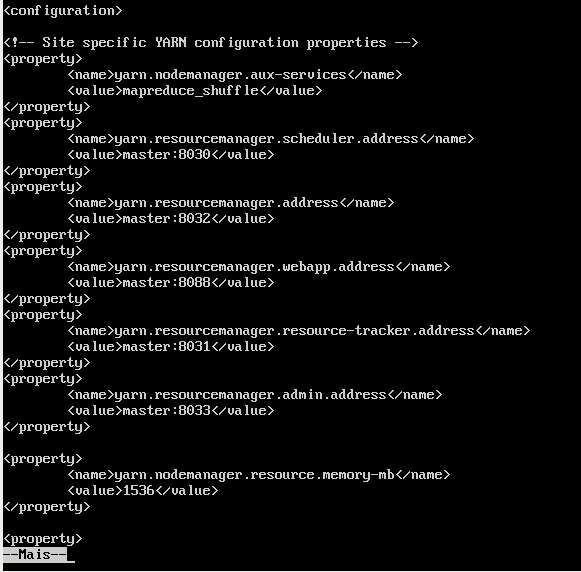
\includegraphics[width=0.80\linewidth]{figures/configYarn-site01}}
	\caption{Configuração do yarn-site.xml}
	\small{Fonte - (proprio autor, 2018)}
	\label{Fig:Configuração do yarn-site.xml}
	\end{center} \end{figure}

\begin{figure}[htbp!] \begin{center}
	% fbox faz uma borda ao redor do seu argumento
	\fbox{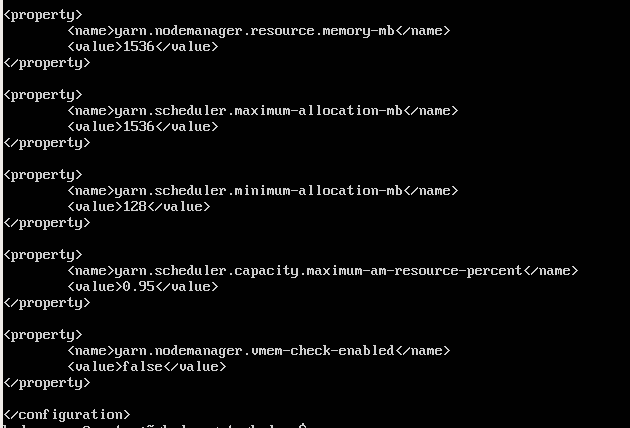
\includegraphics[width=0.80\linewidth]{figures/configYarn-site02}}
	\caption{Configuração do yarn-site.xml}
	\small{Fonte - (proprio autor, 2018)}
	\label{Fig:Configuração do yarn-site.xml-2}
	\end{center} \end{figure}
\end{comment}

\item \textbf{Arquivo de Slaves:} Neste arquivo chamado de \textit{slaves} ele não possui extensão, é o local onde deve-se colocar os nomes das máquinas configuradas no cluster que irão utilizar os serviços do Apache Hadoop. Neste caso o arquivo \textit{slaves} foram acrescentados os seguintes nome: \textit{master}, \textit{slave1}, \textit{slave2} e \textit{slave3}.

\end{itemize}

Após toda a configuração do Apache Hadoop na máquina \textit{master} alguns arquivos precisam ser copiados para os \textit{slaves}, sendo assim, utilizando o comando scp do terminal linux do \textit{master} pode-se copiar os arquivos, core-site.xml, hdfs-site.xml e o yarn-site.xml para os \textit{slaves}. De posse desses arquivos nos diretórios certos, basta executar o seguinte comando: "hdfs namenode -format". Este comando irá formatar o sistema de arquivos, finalizado e com uma mensagem de sucesso. A inicialização do Apache Hadoop pode ser realizada com o seguinte comando: "start-dfs.sh", para isso deve-se está dentro do diretório hadoop/etc/hadoop. Após iniciar o Hadoop é necessário iniciar o Yarn, com o seguinte comando: yarn-start.sh. Feito isso, para saber se está tudo funcionando basta executar o comando jps, como ilustrado nas figuras \ref{Fig:Comando jps Slave} e \ref{Fig:Comando jps Master}.

\begin{figure}[htbp!] \begin{center}
	% fbox faz uma borda ao redor do seu argumento
	\fbox{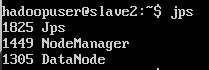
\includegraphics[width=0.40\linewidth]{figures/jpsSlave}}
	\caption{Comando jps Slave}
	\small{Fonte - (próprio autor, 2018)}
	\label{Fig:Comando jps Slave}
	\end{center} \end{figure}
    
    \begin{figure}[htbp!] \begin{center}
	% fbox faz uma borda ao redor do seu argumento
	\fbox{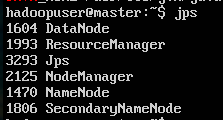
\includegraphics[width=0.40\linewidth]{figures/jpsMaster}}
	\caption{Comando jps Master}
	\small{Fonte - (próprio autor, 2018)}
	\label{Fig:Comando jps Master}
	\end{center} \end{figure}

Como ilustrado na figura \ref{Fig:Comando jps Master}, o nó \textit{master} contém mais processos em relação ao nó \textit{slave}, pois o \textit{master} é o gestor da aplicação, ele irá gerenciar e coordenar as tarefas.

\subsubsection{Cluster Hadoop}

Após completar todas as instalações necessárias, que são desde a criação da primeira máquina virtual até a instalação e configuração do \textit{framework} Apache Hadoop, tem-se o cluster funcionando. Para verificar se o cluster está realmente funcionando foi executado uma tarefa, e a partir de outra máquina acessando o endereço \url{10.0.0.1:8088/cluster/nodes} é possivel navegar e visualizar a interface do Yarn que é executada na porta 8088, enquanto que, o endereço \url{10.0.0.1:50070/dfshealth.html} na porta 50070 é possível visualizar o estado do cluster, como ilustram as figuras \ref{Fig:Interface do Yarn} e \ref{Fig:Estado do Cluster}.

\begin{figure}[htbp!] \begin{center}
	% fbox faz uma borda ao redor do seu argumento
	\fbox{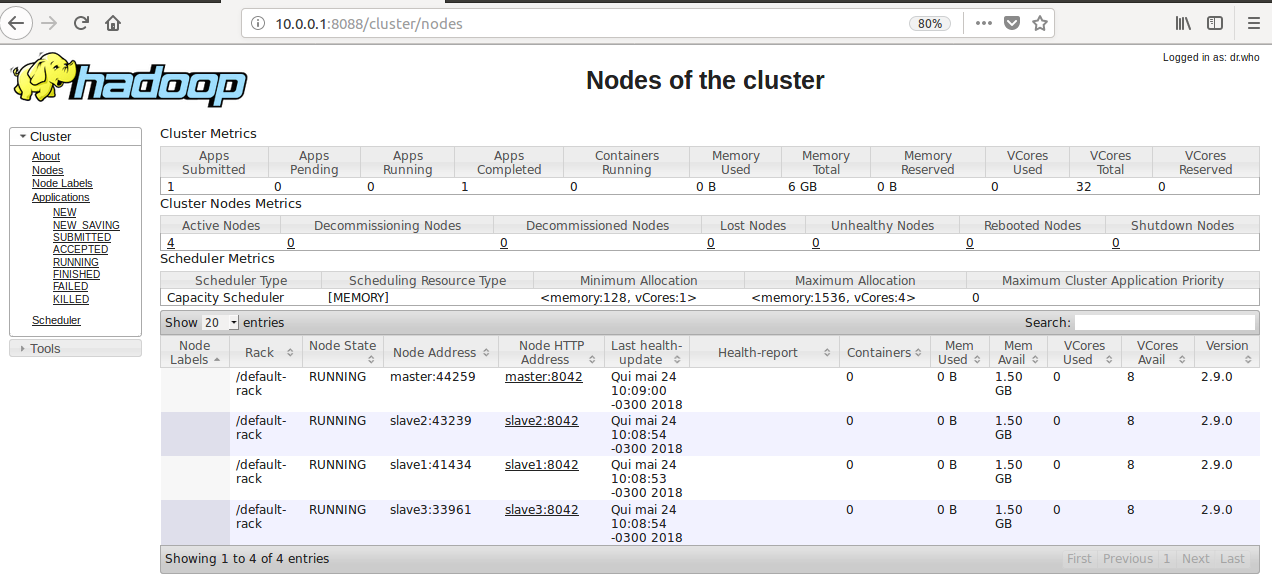
\includegraphics[width=1\linewidth]{figures/interfaceYarn}}
	\caption{Interface do Yarn}
	\small{Fonte - (próprio autor, 2018)}
	\label{Fig:Interface do Yarn}
	\end{center} \end{figure}
    
    \begin{figure}[htbp!] \begin{center}
	% fbox faz uma borda ao redor do seu argumento
	\fbox{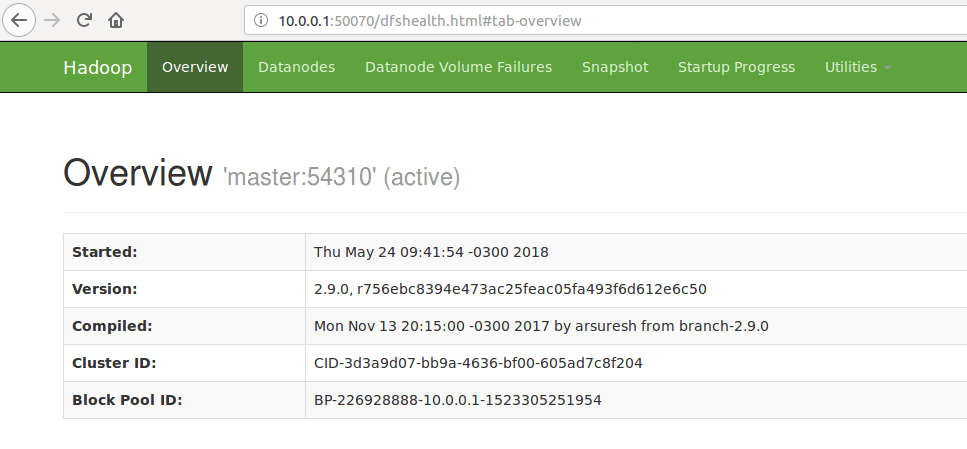
\includegraphics[width=1\linewidth]{figures/estadoDoCluster}}
	\caption{Estado do Cluster}
	\small{Fonte - (próprio autor, 2018)}
	\label{Fig:Estado do Cluster}
	\end{center} \end{figure}


Vale salientar que o acesso as intefaces devem ser realizadas por uma máquina que esteja na mesma rede do cluster. Sendo assim, esse acesso foi realizado pela máquina atacante, que está configurada na mesma rede. Com estes painéis é possível visualizar toda as funcionalidades dos nós, tais como: logs, estatísticas, quantidade de memória disponível e alocada, memória total, quais as tarefas foram executadas sem falhas, e entre outras funcionalidades.
